\documentclass[a4paper,onecolumn,oneside,titlepage,11pt]{article}

\usepackage{tikz}
\usetikzlibrary{shapes,arrows}

% Define block styles for flow diagrams
\tikzstyle{decision} = [diamond, draw, fill=black!20, 
    text width=4.5em, text badly centered, node distance=3cm, inner sep=0pt]
\tikzstyle{block} = [rectangle, draw, fill=black!20, 
    text width=5em, text centered, rounded corners, minimum height=4em]
\tikzstyle{line} = [draw, -latex']
\tikzstyle{cloud} = [draw, ellipse,fill=red!20, node distance=3cm,
    minimum height=2em]


\title{AndroAR: Mobile Augmented Reality application}
\author{Alexandru Damian}
\date{16 June 2012}


\begin{document}
\maketitle
\begin{abstract}
ABSTRACT
\end{abstract}
\tableofcontents

\clearpage
\section{Introduction}
\subsection{Motivation}
\subsection{Structure of thesis}


\clearpage
\section{State of the Art}
Augmented Reality is very popular in the mobile applications industry. However, most applications interact very little with the video feed they overlay the information on. Typically, applications will:
\begin{itemize}
	\item interact with a small part of the current view, such as a \emph{logo} or \emph{banner};
	\item take advantage of the localization capabilities of the phone, such as \emph{GPS positioning} or \emph{compass} and place information on the screen with disregard to what the user's line of sight actually is (\emph{e.g. a user might be facing a wall and be overrun with information, even though he doesn't see anything relevant}.
\end{itemize}
\subsection{Layar}
Layar is a mobile application built for Android and iOS. It is the most well-known augmented reality mobile application in the industry. Having pivoted a few times, it now focuses on bringing the augmented reality experience to printed publications.
\subsubsection*{Disadvantages}
\begin{itemize}
	\item Layar is currently focused on printed publications. One can try to associate a current view of the world (\emph{i.e. what the user sees at a particular moment through the smartphone's camera}) with a \emph{printed magazine page}. However, the world is dynamic and tridimensional, and, therefore, problems will arise when trying to extend the Layar behavior.
\end{itemize}

We must note that Layar has limited support for 3D objects.
\subsection{Google Maps / Street View}
Google Maps enables users to navigate and receive directions on an extremely detailed map. Street View, a subproduct of Google Maps, allows navigation at street view level, allowing the user to asociate information with their surroundings.
\subsubsection*{Disadvantages}
\begin{itemize}
	\item Street View is not live. Street View imagery was captured using dedicated equipment. Efforts are being made to keep the imagery as up-to-date as possible, but this cannot be done all around the world. For example, several areas in Romania contain images that are 4 years old.
	\item Only recently has Street View been offering imagery outside of streets range (\emph{i.e. pedestrian roads, parks, campuses, indoor}
	\item Users can navigate through Street View using their smartphone, but the Street View imagery will completely replace what the user sees. This will result in \emph{lower accuracy} and \emph{higher bandwith usage}.
\end{itemize}
\subsection{Wikitude}
\subsection{Mixare}

\clearpage
\section{Goals for AndroAR}
While designing AndroAR, we focused on several keywords:
\subsection*{Live}
We need to focus on displaying information relevant to what the user sees, not just to the user's position and orientation. Most augmented reality applications will place an overlay of information on top of the current camera feed; the two are related only by the current localization features of the user (\emph{i.e. GPS position, compass orientation}) and not by what the camera feed actually shows.

\textbf{Layar} offers a live view, but is only focused on paper.

\textbf{Street View} doesn't offer a live view, but Google Maps supports uploading of user images and tagging; these images can be augmented onto the Street View imagery, but that only works on the desktop web version.
\subsection*{Fast}
Using the camera feed brings some issues regarding speed and bandwidth since displaying information is not a matter of only querying a database with the user's current position anymore. We need to find a way to divide the computational effort between the server and the mobile application. We must also consider the effect of latency on the query replies (\emph{i.e. by the time the user receives the query reply, the detected objects might have translated).}

By its design, \textbf{Layar} users will wait for the reply to the query. A typical usecase of Layar is: \emph{a user will see the message \emph{Scan for a behind-the-scenes video of the article} on the cover of a magazine and will wait for the application to serve the video}.

Since it's not live, \textbf{Street View} can precache the information it needs in order to serve information to the user. Queries will not be affected by what the users see, but only by their position.

\subsection*{Correct}
We must make sure that the information (\emph{i.e. objects associated with images and metadata}) is correct. Since we are using a crowdsourced approach, we should consider rating of images to allow removal of incorrect associations. Also, we must deal with spam.

\textbf{Layar} has fewer problems with this since they are using a business-to-consumer model, in which the information is provided by the business and the queries are made by the consumer (\emph{i.e. a magazine creates the layers and the buyer uses the application}. Layar can correctly assume that business will provide high-quality information.

\textbf{Street View} already has correct and high-quality imagery. Images added by users can easily be filtered by first querying them against their database.

\clearpage
\section{Application Workflow}
A user can interact with our application in two ways:
\begin{enumerate}
	\item by making queries while using the application;
	\item by sending images annotated with objects and metadata.
\end{enumerate}
We will illustrate the overall workflow for each of them below.

\subsection{Queries}
Let us assume that at one point in time, while the user is using the application, the applicatin needs to find all the objects that appear in a frame, along with their metadata. To accomplish this, we will send a request to the server that will be completed in 6 steps:
\begin{enumerate}
	\item The mobile application will encapsulate the current frame, along with localization information (GPS position and compass orientation) and send it to the server;
	\item The server will forward the query to the database which will fetch from storage, all the possible objects in the user's line of sight.
	\item The database will return the objects that might pe present in the frame. For each object, information that will help match the particular object to an image will also be returned. Note that each object may (and should) be present in more than one image. We will return matching information for the best performing fraction of these images. The information we return may contain:
	\begin{enumerate}
		\item image features (\emph{e.g. lines, corners, areas of constrast, etc.});
		\item illumination information;
		\item etc.
	\end{enumerate}
	\item We will forward the initial query, along with the possible objects to the image recognition component. This component will:
		\begin{enumerate}
			\item compute the features for the query image;
			\item compare the features for the query image to the features of every possible object and assign a rate of success (or certainty) to each statement
			
			$X$ is present in the query image $I$, where $X$ is a $possible\:object$
		\end{enumerate}
		\item Using a threshold for the rate of success, we will end up with a subset of the possible objects being classified as detected objects. These detected objects, along with the corresponding positions in the query image will be sent back to the server by the image recognition component.
		\item The server will then forward the reply to the mobile application.
\end{enumerate}

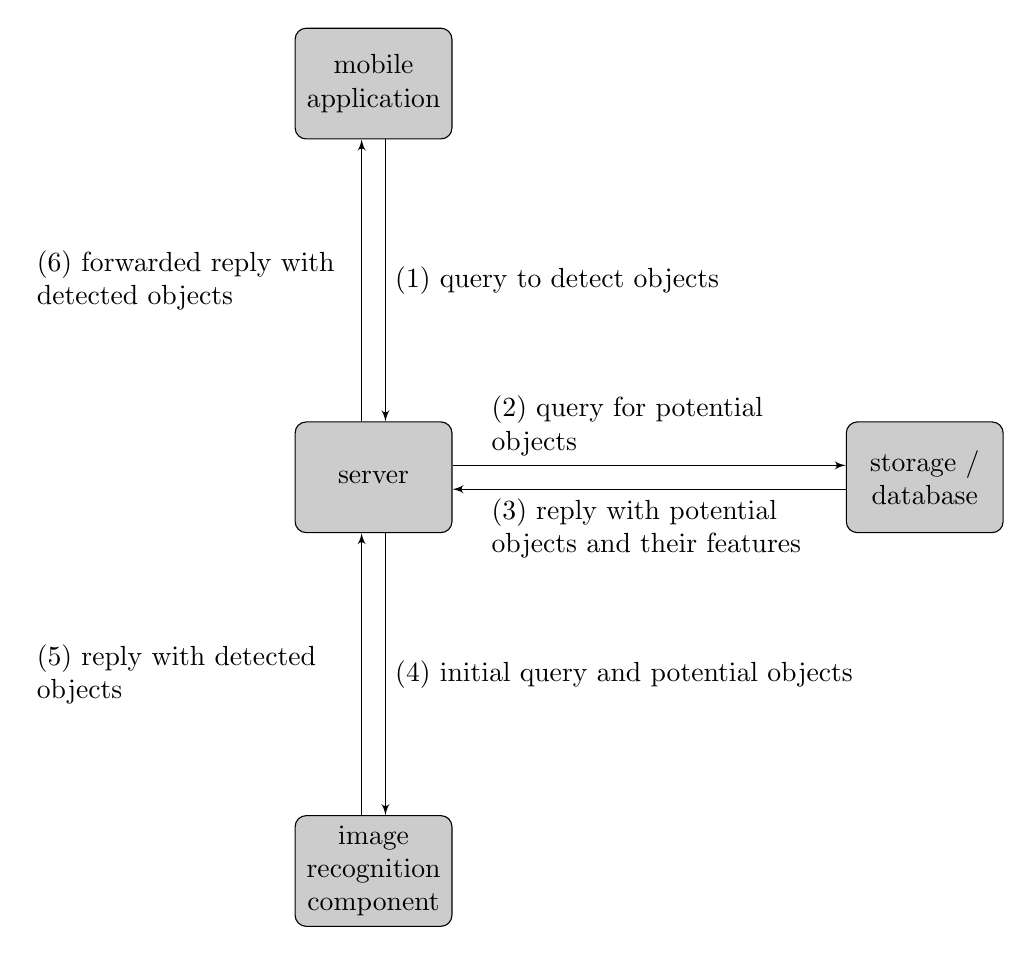
\begin{tikzpicture}[node distance = 2cm, auto]
    % Place nodes
    \node [block] (app) {mobile application};
    \node [block, below of=app, node distance=5cm] (server) {server};
    \node [block, right of=server, node distance=7cm] (db) {storage / database};
    \node [block, below of=server, node distance=5cm] (ai) {image recognition component};
    % Draw edges
    \path [line] ([xshift=1ex]app.south) -- node [text width=6cm] {(1) query to detect objects} ([xshift=1ex]server.north);
    \path [line] ([yshift=1ex]server.east) -- node [text width=4cm] {(2) query for potential objects} ([yshift=1ex]db.west);
    \path [line] ([yshift=-1ex]db.west) -- node [text width=4cm] {(3) reply with potential objects and their features} ([yshift=-1ex]server.east);
    \path [line] ([xshift=1ex]server.south) -- node [text width=6cm] {(4) initial query and potential objects} ([xshift=1ex]ai.north);
    \path [line] ([xshift=-1ex]ai.north) -- node [text width=4cm] {(5) reply with detected objects} ([xshift=-1ex]server.south);
    \path [line] ([xshift=-1ex]server.north) -- node [text width=4cm] {(6) forwarded reply with detected objects} ([xshift=-1ex]app.south);
    
\end{tikzpicture}

\subsubsection*{Example}
We will illustrate the previous workflow with an example:
\begin{itemize}
	\item Let us assume that a tourist is travelling through Paris and, when a query is made to the server, he is looking at the \emph{Eiffel Tower}.
	\item The server will receive a query containing an image of the \emph{Eiffel Tower}, along with the tourist's position and orientation. 
	\item The server will then request from the database, the possible objects that might be present in the tourist's line of sight. For example, the server might request the top (at most) 10 ranking instances of all the objects in a 1 kilometer radius and in a 90\% cone in front of the user.
	\item A possible reply from the server contains the features for 10 images of the \emph{Eiffel Tower} and the features for 6 images of \emph{Les Invalides}.
	\item These will be forwarded to the image recognition component which will try to match 2 possible objects with the query image. The confidence rates that result can be:
		\begin{center}
			\begin{tabular}{|c|c|}
				\hline
				\textbf{Object} & \textbf{Confidence}\\
				\hline
				Eiffel Tower & .85\\
				Les Invalides & .5\\
				\hline
			\end{tabular}
		\end{center}
	\item With a threshold of $.75$, only the \emph{Eiffel Tower} will be selected as a valid match and that will be returned as the query reply.
\end{itemize}

\subsection{Store requests}
Our application supports and encourages crowd-sourced contributions to annotate new landmarks. Should a user want to annotate a landmark, the application will allow them to freeze on a particular frame, create  bounding boxes around the landmarks and annotate them with information. We will need to store this information into our database.
The application will send the current frame, the localization features (GPS position and orientation), the cropped images associated with the landmarks and their information to the server (1), which will forward it to the database (2). After storing this information, the server will send a request to OpenCV to compute the features for the cropped images, in order to also store them in the database (3). The reply that is received (4) is forwarded to the database (5).

\section{Bibliography}
\begin{thebibliography}{99}
\bibitem{first}FIRST BOOK
\end{thebibliography}

\end{document}